\subsection{Architecture Globale}

\subsubsection{Interfacage}

\subsection{Module taxonomique}

\begin{figure}[h!]
  \centering
  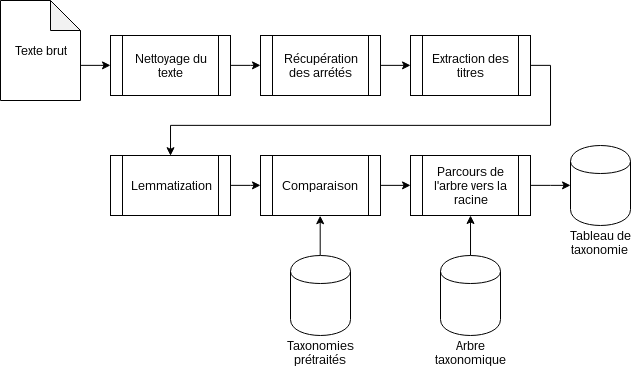
\includegraphics[width=0.8\textwidth]{diagArchiTaxo.png}
	\caption[]{Diagramme de l'architecture du module taxonomique}
  \label{}
\end{figure}


Le module taxonomique a pour charge d'extraire et d'assigner une ou plusieurs taxonomie a un document. Pour des raisons d'efficacité et de précision, ce module extrait d'abord le titre des arrêtés administratifs contenu dans le texte, puis les compare avec les taxonomies après une normalisation. Cette normalisation consiste en un nettoyage des accents et caractères spéciaux, ainsi qu'une lemmatization, procédure où l'on remplace un mot par sa racine. Ces opérations permettent une comparaison plus robuste et moins dépendante du contexte de la phrase. 

Pour chaque mot de la taxonomie, le module va vérifier si celui ci est présent dans le titre qu'il est en train d'analyser. Si oui, ce mot est ajouté a la taxonomie du document.

Pour obtenir une taxonomie plus vaste, nous prennons également en compte la structure de la taxonomie. En effet, celle ci se présente sous forme d'un arbre. Chaque sections possèdes des sous sections, qui permettent un affinage et une grande précision dans la classification. L'idée principale étant de considérer que si un document possède comme taxonomie une feuille ou un noeud de cette arbre, alors il doit nécessairement posséder comme taxonomie tout les parents de ce nœud. Nous remontons donc jusqu'a la racine de l'arbre depuis le noeud, en ajoutant a la taxonomie du document tout les noeuds que nous rencontrons en chemin.
\begin{figure}[h!]
  \centering
  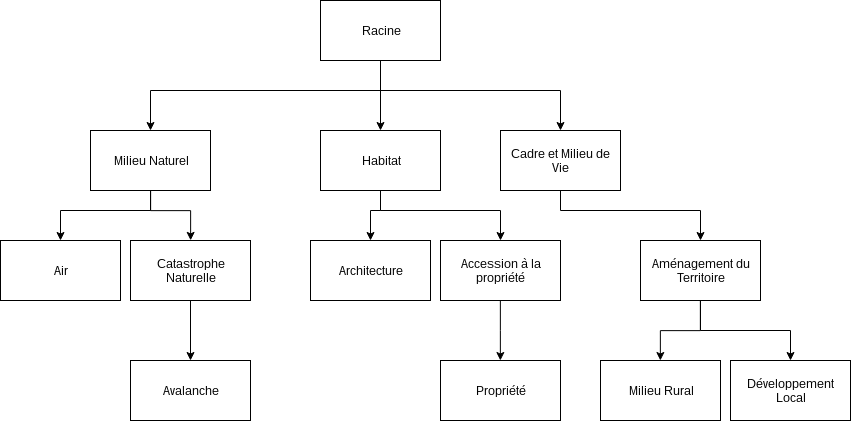
\includegraphics[width=0.8\textwidth]{TaxoTree.png}
	\caption[]{Apercu de l'arbre taxonomique}
  \label{}
\end{figure}
